\section{Proposal's context, positioning and objectives}
\label{sec:context}

\subsection{Objectives and scientific hypotheses}
\label{sec:goals}

\Comments{Present the objectives and the research hypotheses ; present the scientific and technical barriers to be lifted ; present the expected results; if applicable describe any final products developed.}

\noindent\textbf{Context.}
3D volumes come from the segmentation of magnetic resonance, X-ray tomographic or micro-tomographic images. 
They are also generated in scientific modelling and by voxel editors. 
This project is about the geometry of volume boundaries, called \emph{digital surfaces} (fig.~\ref{fig:snow}). 
Keeping the digital nature of the data is an advantage
to use efficient spatial data structures such as voxel octree, 
to perform constructive solid geometry operations,
to do integer-only and exact computations, etc.
A drawback is its poor geometry, because at any resolution a digital surface is only 
made up of quadrangular surface element (\emph{surfel} for short) 
whose normal vector is parallel to one axis. 
Many tasks in computer graphics, vision and 3D image analysis require a richer geometry: 
rendering, surface deformation for simulation or tracking, precise geometric measurements, etc.
To perform relevant geometric tasks and 
to benefit from the above-mentioned advantages in the same time, 
we need to enhance the geometry of digital surfaces by estimating extra data for each surfel. 
This project focuses on estimations of local and first-order geometric quantities
such as normal vector direction.
%%, distance to boundary, coverage of the inner and outer incident voxels 
%%(see fig.~\ref{fig:2D} for a 2D illustration).  

\begin{figure}[hb]
  \centering
%
%\subfloat[]{ 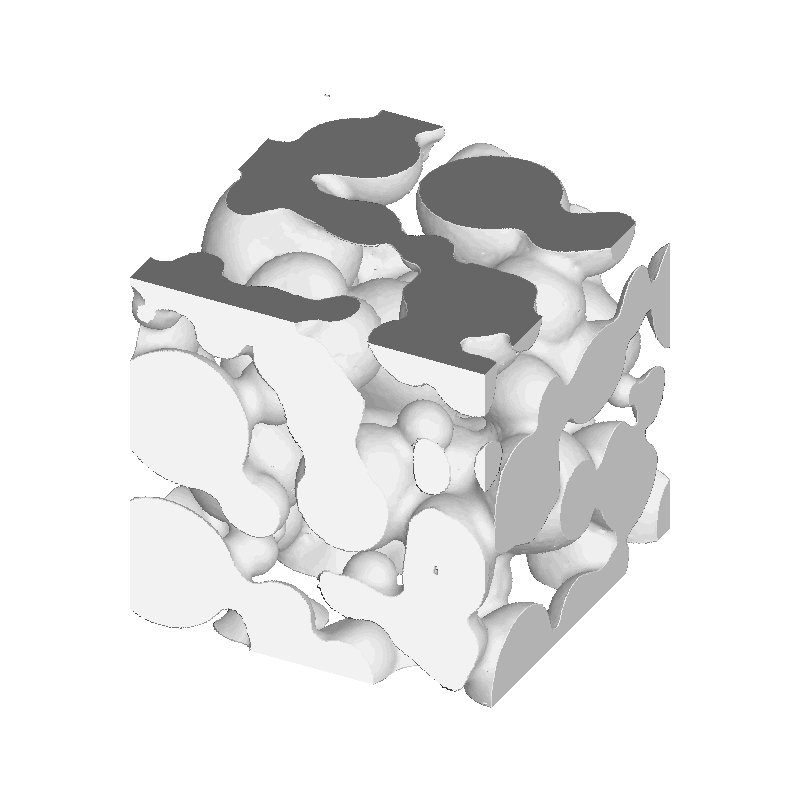
\includegraphics[height=0.2\textheight]{INH5_512_0}}
%
\subfloat[]{
\begin{tikzpicture}[spy using outlines={circle,yellow,magnification=2.5,size=2.8cm,connect spies}]
\node {\includegraphics[width=0.45\textwidth]{closeup-normals-3710x2112}};
\spy on (1.2,-0.2) in node [left] at (-0.95,-0.75);
\end{tikzpicture}
}
%
%
\subfloat[]{
\begin{tikzpicture}[spy using outlines={circle,yellow,magnification=2.5,size=2.8cm,connect spies}]
\node {\includegraphics[width=0.45\textwidth]{closeup-facets-3710x2112}};
\spy on (1.2,-0.2) in node [left] at (-0.95,-0.75);
\end{tikzpicture}
}
%
\caption{``ice-air'' interface in a micro-tomographic image of
  snow\protect\footnotemark. Local normal vectors are estimated
  at each corner (a) by computing relevant facets (b).} 
\label{fig:snow} 
\end{figure}
\footnotetext{obtained by the 3SR Lab and CEN/CNRM - GAME URA 1357/M\'{e}t\'{e}o-France - CNRS, 
shared during ANR-11-BS02-009 DigitalSnow project.}

\noindent\textbf{Scientific bottleneck.}
The surface geometry within a patch around each surfel should be gathered to provide such estimations
-- \eg by polynomial fitting \cite{Cazals2005,Cazals2008}.
Almost all methods require at least one parameter that controls the size of the patch.  
On the other hand, this project aims at providing \emph{accurate} and \emph{parameter-free} estimators
based on a surface patch with \emph{adaptive} size.
%Note that accuracy will be evaluated in a \emph{multigrid-convervence} framework as described in section \ref{sec:wp}, WP2. 
Since we are looking for first-order estimations, the patch will be typically a piece of digital plane
that locally fits to the digital surface. %(fig.~\ref{sub:pattern}).
A challenge is to cover the whole digital surface by maximal pieces of digital plane. 
What makes the problem hard is that there is a combinatorial explosion
of maximal pieces of digital plane \cite{Sivignon2009} and that among them,
not all are tangent to the digital surface in a point set framework.  
An opportunity to make a breakthrough in this issue is the recent development
by the principal investigator and its collaborators of \emph{plane-probing}
algorithms \cite{LPRTCS2016, LPRDGCI2016, LPRJMIV2017}. These algorithms decide
on-the-fly how to probe the digital surface and make grow a piece of digital plane,
which is tangent by construction. The growth direction is given by both arithmetic and geometric properties.

\noindent\textbf{Objectives and expected results.}
This project aims at analyzing digital surfaces. Three distinct goals can be highlighted:
\begin{enumerate}
  \item[(G1)] 
The first goal of this project is to study extra arithmetic and combinatorial properties
of plane-probing algorithms. We expect to design an ultimate plane-probing algorithm that
only probes a part of digital surface \emph{as small as possible} to provide a relevant facet.
A formal definition of what is meant by \emph{small} and a theoretical upper bound should be given.
In addition, we expect to correctly process non-convex parts by generating an underlying
minimal and connected piece of digital plane. 
%(see WP0 and WP1 in section~\ref{sec:wp}, describing work packages).
 \item[(G2)]
The second goal is to derive \emph{efficient}, \emph{accurate} and \emph{parameter-free} estimators
of \emph{local} and \emph{first-order} geometric quantities: normal vector (and surfel area as a by-product),
distance to boundary, voxel coverage (fig.~\ref{fig:2D}). We expect to derive such estimators from
the above-mentionned plane-probing algorithm and provide a theoretical evaluation of their accuracy
with respect to resolution.  
%(WP2).
 \item[(G3)]
The third goal is to provide a method and a tool for an automatic and \emph{multiscale} analysis of digital surfaces,
based on the number or the size of the computed facets for several subsampled versions of the input 3D volume. 
We expect to develop a tool that provides, without any parameter, the scale at which noise is unlikely. Based on
this tool, we may add other features like a 3D normal estimator robust to noise.  
%(WP3). 
\end{enumerate}

\begin{figure}[hbt]
  \centering
\subfloat[]{ 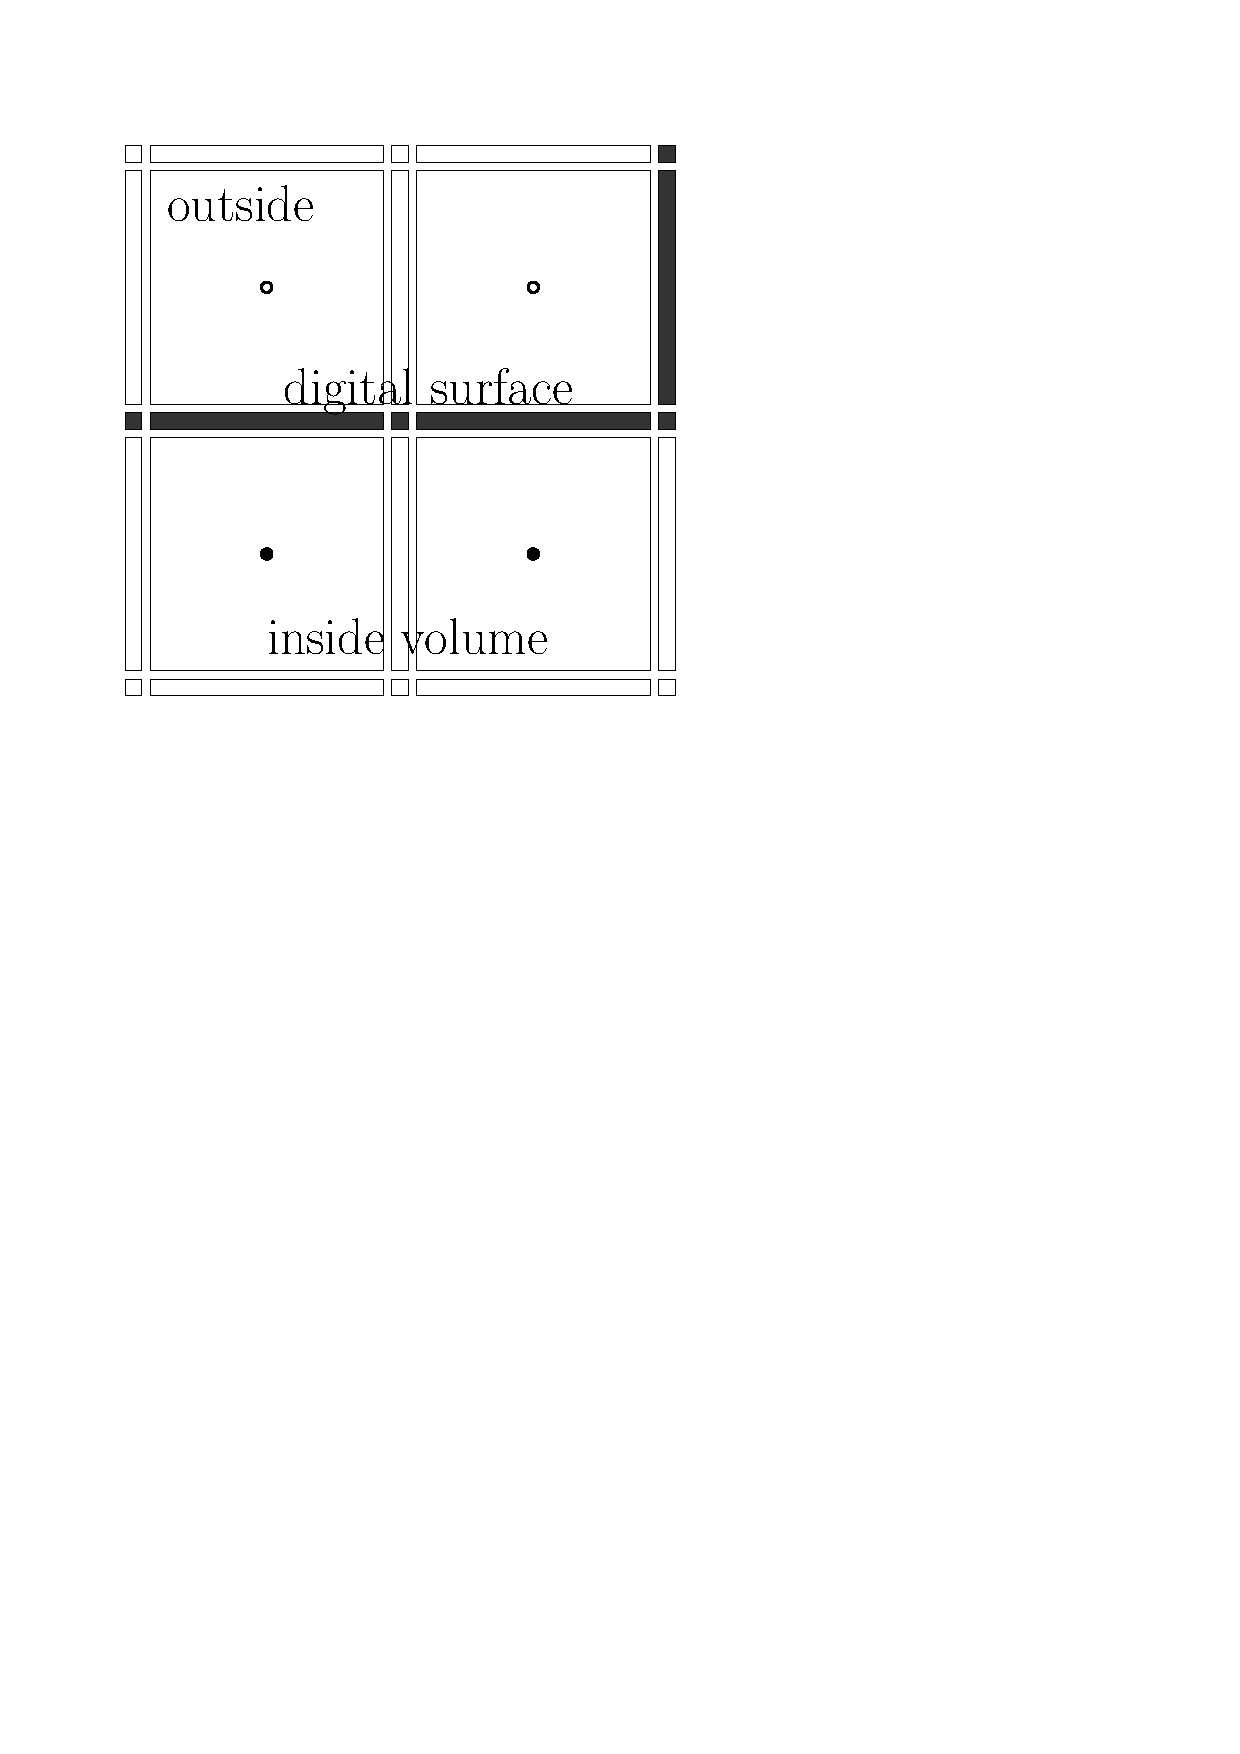
\includegraphics[width=0.13\textwidth,page=1]{square.pdf} } \hspace{0.05\textwidth}
\subfloat[]{ \includegraphics[width=0.13\textwidth,page=2]{square.pdf} } \hspace{0.05\textwidth}
\subfloat[]{ \includegraphics[width=0.13\textwidth,page=3]{square.pdf} } \hspace{0.05\textwidth}
\subfloat[]{ \includegraphics[width=0.13\textwidth,page=4]{square.pdf} } 
 \caption{2D illustration of a digital surface: voxels are big squares whose center is depicted by a black (resp. white) disk if it lies inside (resp. outside) the volume; surfels are elongated dark rectangles. We want to estimate a relevant normal vector at a given surfel (b), but also locally reconstruct a boundary perpendicular to this normal vector in order to derive distance and coverage estimations (c-d).} 
\label{fig:2D} 
\end{figure}

 % at T+24 ?
New algorithms, theoretical results and experimental studies will be gathered in papers submitted to
top venues or in peer-reviewed international journals. Plane-probing algorithms and derived estimators
 will be implemented in \DGtal, tools in \DGtalTools~ with an \IPOL~ companion paper. 

%\todo{expected results and final products}

%1-WP0: algorithm purely local, from any starting point, which leads to a reduced basis and retrieves any normal
%1-WP1: pattern generation: minimal number of tiles, connected, 
%2-WP2: estimateur + ordre de convergence theorique + applis ?
%3-WP3: outils qui prend un volume et sors un sous-échantillon non bruité, ou un ensemble de voxels à différentes tailles (publi IPOL)
%=> for each publication and implementation in DGtal. 

%transition not relevant here
%Since there are so many perspectives and paths to follow, this project needs to strengthen a team of experts by full-time workers in order to make the best of them. 

\subsection{Originality and relevance in relation to the state of the art}
\label{sec:art}

\Comments{Emphasise the ambitious nature of the proposal and the novelty of the research in relation to the state of the art ; show the possible contributions of project partners to the state of the art ; present any preliminary results. In the case of a project proposal following up on previous project(s) already funded by ANR or by another body, provide a summary of the results achieved and clearly describe the new issues raised and the new objectives set out in the light of the earlier project.}

In this section, we underline the novelty of the proposed approach in relation to the state of the art.  
We focus on the estimation of the normal direction, which is the most challenging task with the biggest impact. 
Other first-order quantities are either obtained as a by-product of the normal estimation (\eg surfel area)
or carry position information already approximated by the digital surface itself (\eg distance to boundary).
%In this last case, it seems unlikely that the accuracy could be improved by an order of magnitude. 

In addition, a digital surface is a quadrangular mesh. The vertex set consists of evenly spaced data points
whose coordinates are (half-)integer. This specific point cloud approximates a continuous 2-manifold under a
uniform noise model due to discretisation errors. That is why we review the most common methods for normal estimation
not only on digital surfaces, but also on meshes and point clouds.
%TODO nombreuses applications de normal estimation ce qui explique qu'il y ait beaucoup de travaux.  

%% Note that we do not present 2D estimators (\eg \cite{Provot2011,Esbelin2011,Esbelin2016}),
%% with the exception of \cite{Lachaud2007}, which is parameter-free and used in 3d estimators
%% \cite{Lenoir1996,Tellier1999,Lachaud2003}. 

Since one goal of the project is to propose an accurate and parameter-free normal estimator,
we focus in this state of the art on user-defined parameters and, for digital surfaces only,
we check if the estimator is \emph{multigrid-convergent}, \ie the smaller the grid step,
the higher the resolution, the more accurate the estimator. 


%% \noindent\textbf{Digital surface and multigrid convergence.}

%% 3D volumes are collections of cubes. % of size $h$, called \emph{grid step}. 
%% Their topological boundary is a quadrangular mesh called \emph{digital surface}.
%% The vertex set consists of evenly spaced data points whose coordinates are
%% half-integer. This set approximates a continuous 2-manifold under a uniform
%% noise model. 
%% %TODO: Lachaud Thibert

%% Most of the time, when we are working with a digital surface, we are 
%% interested in the geometry of a continuous shape whose digitization
%% is the input 3D volume.
%% Formally, given a compact shape $X \subset \R^3$,
%% its digitization at grid step $h \in \R^+$ is $\Dig(X) := \{z \in \Z^3, hz \in X\}$.
%% If we denote the axis-aligned closed cube centered on $z \in h\Z^3$ and of size $h$ as $Q_z^h$,
%% the cube embedding of a digital set $Z$ at grid step $h$ is $\underset{z\in Z}{\cup}Q_z^h$.
%% Let $\partial_h X$ be the topological boundary of the embedding of the digitization of $X$: 
%% \[
%% \partial_h M := \partial \Big( \underset{z\in\Dig(X)}{\bigcup}Q_z^h \Big).
%% \]

%% We expect that a given geometric quantity, such as a normal vector,
%% computed at a point of a digital surface ($\partial_h X$),
%% is close to the one of the underlying continuous shape ($X$) at a close enough point. 

%% \begin{Definition}[multigrid-convergent estimator \cite{Coeurjolly2012}]
%%   \label{def:multigrid-convergence2}
%%   The estimator $\hat{Q}$ is {\em multigrid-convergent} for the family
%%   {\Shapes} if and only if, for any shape $X \in \Shapes$,
%%   there exists a grid step $h_X>0$ such that the estimate
%%     $\hat{Q}(\Dig(X),y,h)$ is defined for all
%%   $y \in \partial_h X$ with $0<h < h_X$, and for any $x \in \BT{X}$,
%%   \begin{equation*}
%%     \forall y \in \partial_h X \text{~with~} \| y - x \|_1 \le h, \quad
%%     \hat{Q}(\Dig(X),y,h) - Q(X,x) | \le \tau_{X,x}(h),
%%   \end{equation*}
%%   where $\tau_{X,x}: \R^{+*} \rightarrow \R^+$ has null limit at
%%   $0$.
%%   %% This function defines the speed of convergence of $\hat{Q}$
%%   %% toward $Q$ at point $x$ of $\BT{X}$. The convergence is {\em uniform} for
%%   %% $X$ when every $\tau_{X,x}$ is bounded from above by a function
%%   %% $\tau_X$ independent of $x \in \BT{X}$ with null limit at $0$.
%% \end{Definition}

%% The accuracy of a multigrid-convergent estimator depends on the grid step:
%% the smaller the grid step, the more accurate the estimator. 

\subsubsection{Normal estimation on point clouds, meshes and digital surfaces}
\label{sec:estim:all}

TODO: dire quel est l'interet d'estimer des normales ?

\noindent\textbf{Fitting.}
\citeauthor*{Hoppe1992} estimate the normal at a given data point by computing
the least squares best fitting plane to a point set within a neighborhood
around the point of interest \cite{Hoppe1992}.
Other fitting surfaces have been used too, such as jets, \ie truncated Taylor expansion
of a surface expression \cite{Cazals2005,Cazals2008}. 

All fitting methods first consist in collecting the points used for the fitting.
In the mesh case, a breadth-first search visit the neighbors until enough points
have been collected. In the point-cloud case, we typically resort to the k-nearest-neighbors
strategy. In both cases, the number of points to collect is usually a user-defined parameter,
even if some heuristics are proposed to select it automatically \cite{Hoppe1992,Cazals2005}.  

%\cite{Provot2011} ?

%In 3d, a straightforward application
%of \cite{Cazals2005}[Theorem 3] to digital surface shows that a polynomial fitting of degree $n$
%estimates the coefficients of the unit normal vector in $O(h^n)$.
%TRIS probablement faux

\noindent\textbf{Voronoi diagram.}
Instead of approximating the tangent space, another familly of methods focuses on the
Voronoi diagram to estimate at best the orthogonal space. \citeauthor*{Amenta1999} first use the
furthest vertex of the Voronoi cell to estimate the normals of point clouds \cite{Amenta1999}.
In order to get more stable estimates, \citeauthor*{Alliez2007} propose to apply linear fitting
to the Voronoi cell or to the union of Voronoi cells into a neighborhood \cite{Alliez2007}. 
\citeauthor*{Merigot2011} propose an improvement %, called Voronoi Covariance Measure (VCM),
by taking a weighted average of covariance matrices of Voronoi cells instead of
taking the covariance matrix of their union \cite{Merigot2011}. In their method,
only the intersection between the Voronoi diagram and a ball around the data point
are taken into account in order to get purely local information about the surface geometry.
A digital variant has been proposed by \citeauthor*{Cuel2015} \cite{Cuel2015}. 

\noindent\textbf{Integral invariants.}
In the mesh case, another method sums up the surface geometry within a ball by 
computing integrals over the intersection between the ball and the volume
bounded by the mesh \cite{Pottmann2009}. The covariance matrix of the intersection set 
provides a way to estimate principal curvatures, principal directions and normal direction.
A digital variant has been proposed by \citeauthor*{Lachaud2017} \cite{Lachaud2017}.

Note that the ball radius is a user-defined parameter in these methods. The above-mentionned
digital variants \cite{Cuel2015,Lachaud2017} are multigrid-convergent for digitization
of smooth shapes if the radius is conveniently chosen with respect to the grid step.

\noindent\textbf{Convolution.}
TODO ?
%pas d'isotropie, donc filtres
%bilateral mesh denoising
%\cite{Fourey2009}
%\cite{Esbelin2011,Esbelin2016})

\noindent\textbf{Randomized Hough Transform.}
To end, let us mention also probabilistic methods based on the Randomized Hough Transform.
Boulch and Marlet consider many random triples of data points in a neighborhood
and bin their normal direction into a spherical histogram \cite{Boulch2012}.
Maximal vote provides the normal estimate. However, their method has many input parameters,
the first of which is the size or radius of the neighborhood. 

\subsubsection{Parameter-free normal estimators on digital surfaces}
\label{sec:estim:ds}

All previous methods require at least one parameter that controls the size of the neighborhood.
On the other hand, the specificity of digital surfaces makes the development of parameter-free
estimators possible. The trick is to perform a uniform fitting of the data points by a plane.
In addition, instead of specifying the number of data points \emph{a priori}, they are added
step by step, while a maximal admissible error is not reached. This threshold is not a user-defined
parameter, but a known constant, because the data points follow a known uniform noise model
in case of digital surfaces. In 2D, methods based on digital straight segments (DSSs) follow
this approach.

The set of maximal DSSs, \ie inextensible straight parts, can be computed by one scan of the
digital curve \cite{Feschet1999,Feschet2005} and provides a parameter-free and multigrid-convergent
tangent (and normal) estimator \cite{Lachaud2007}.
This estimator preserves the inflexion points because maximal DSSs are closely related to
local convexity \cite{Roussillon2011} and normal integration over the digital curve yields
a multigrid-convergent length estimator \cite{Coeurjolly2004}. 
In addition, asymptotic properties of maximal DSSs can be used to estimate the local amount
of noise along the digital curve \cite{Kerautret2012}.  

In higher dimension, to the best of our knowledge, only one parameter-free normal estimator
has been proposed in 3D \cite{Lenoir1996,Tellier1999} and extended to nD \cite{Lachaud2003}.
It is based on maximal DSSs on 2D slices. Maximal DSSs provide windows of adaptive size
but the slicing truncates the geometric information and leads to
an artificial spatial variability because two neighbor surfels only
share one slice over two. 

Given an estimator with an input size parameter, a general strategy to automatically and adaptively select
the parameter value consists in taking the size of maximal DSSs. 
The idea of such hybrid method has been used first in \cite{Devieilleville2009}
for a comparative study of 2D normal estimators and then in \cite{Coeurjolly2014IIfree}
for mean curvature estimation by integral invariants.
In 2D, this strategy is quite interesting for higher-order estimators such as curvature,
but is totally disproportionate for normal estimation since maximal DSSs straightforwardly give a good estimator. 
In 3D, even if this hybrid method may be useful for normal estimation, its computation cost may be rather high,
because we must take into account the preprocessing cost to approximate the parameter value for each surfel,
and the cost of the original estimator without any optimization trick that takes profit of the neighboring
computations with the same parameter value, as done in \cite{Lachaud2017}. 

Finally, another possible approach is to mimic the 2D tool box by computing the set of
digital plane segments (DPSs) that locally fits to the digital surface. This approach
has been used for surface area estimation \cite{Klette2001}, reversible polyhedrisation
\cite{Sivignon2004} and normal estimation \cite{Charrier2011}.
The challenge is to find how to scan the digital surface to efficiently recognize relevant DPSs. 

TODO: discuter \cite{Charrier2011} et en donner des limitations ?

\subsubsection{Digital plane segments: recognition and generation}
\label{sec:dps}

\noindent\textbf{Recognition of digital plane segments.}
A \emph{digital plane} is an infinite digital set that 
consists of several consecutive and parallel layers of coplanar points. 
It is defined by a (nonzero) normal $\vec{n} \in \Z^3$ and a position $\mu \in \Z$ as follows
\cite{reveilles1991}:  
\begin{equation}
  \label{eq:plane}
\Plane{\mu}{\vec{n}} := \{ \vec{x} \in \Z^3 \ | \ \mu \leq \vec{x} \cdot \vec{n} < \mu + \|\vec{n}\|_1 \}.
\end{equation}

Given a finite digital set $\Set$, the \emph{recognition problem} consists in providing
$\mu$ and $\vec{n}$ such that $\Set \subseteq \Plane{\mu}{\vec{n}}$ if any.
Note that such a recognition problem can have zero or infinitely many solutions.
One solution can be found in linear time, \ie in $O(|\Set|)$, by linear programming
and all solutions can be found in $O(|\Set|\log{(|\Set|)})$ by computational geometry tools.
See \cite{Brimkov2007} for a review on digital planarity.

However, we usually want to add data points step by step and incrementally update the solution
or the set of solutions. In this on-line framework, algorithms with optimal bounds are difficult
to implement and are in all probability slow in practive due to a high constant (see for instance
\cite{Buzer2003}).
On the other hand, there exists fast geometrical algorithms but with higher theoretical bounds,
\eg \cite{Gerard2005, Charrier2008, Veelaert2012}.
%\cite{Gerard2009} preimage
%\cite{Stojmenovic1991} separation
%Provot2006, largeur

Actually, the main challenge is not so much to recognize DPSs, but more to find which data points
should be taken into account during the recognition process to obtain DPSs tangent to the digital
surface. In addition, as noted \cite{Charrier2011}, most inextensible digital planar sets are not
characteristics of the local geometry of the shape and finding the smallest subset which covers
the digital surface has been shown to be NP-complete \cite{Sivignon2009}.

Segmentation methods usually make grow a point set from a seed by a breadth-first search according
to some heuristics and decide whether the current set is a piece of digital plane or not
(see for instance \cite{Klette2001} or \cite{Sivignon2004}). 
%\cite{Provot2009} un peu different car parametre de bruit
The results are however highly dependent on the chosen heuristics.   

Until recently, artihmetic properties of digital planes did not help so much.
Pionneering incremental recognition algorithms based on arithmetic properties
\cite{Debled1994,Mesmoudi2002} are neither as easy-to-implement nor as fast as
purely geometric ones, such as \cite{Gerard2005}.  
The work of V. Berth\'{e} and T. Fernique \cite{Fernique2009,Berthe2011}, 
based on multidimensional continued fractions and desubstitution on words,
is quite interesting from a theoretical point of view. However, their algorithm,
which reduces a piece of digital surface until no transformation is possible,
is not of practical interest because it requires the whole point set to be known
in advance and must be coupled with another recognition algorithm to conclude
at the last step.  

\noindent\textbf{Preliminary results: plane-probing algorithms.}
An opportunity to make a breakthrough in this issue is the recent development
by the principal investigator and its collaborators of \emph{plane-probing
algorithms} \cite{LPRTCS2016, LPRDGCI2016, LPRJMIV2017}. 
Given a digital plane $\Plane{\mu}{\vec{n}} \subset Z^3$
and a starting point $\vec{p} \in \Set$, 
a plane-probing algorithm computes the parameters of a digital plane $\Plane{\mu'}{\vec{n}'}$
containing $\vec{p}$ by sparsely probing $\Plane{\mu}{\vec{n}}$ with the predicate
``is $\vec{x}$ in $\Plane{\mu}{\vec{n}}$?''. The parameters of $\Plane{\mu}{\vec{n}}$
and $\Plane{\mu'}{\vec{n}'}$ are expected to be equal when the algorithm terminates.
%for any $\vec{p} \in \Plane{\mu}{\vec{n}}$. 

What makes plane-probing algorithms promising is that they decide on-the-fly how
to probe the digital surface and make grow a piece of digital plane, which is
tangent by construction. 
The first algorithm of this kind has been proposed in \cite{LPRTCS2016}.
Its principle is to deform an initial unit tetrahedron based at the starting point
with only unimodular transformations. Each transformation is decided by looking
mostly at a few points around the tetrahedron. These points are chosen so that
the transformed tetrahedron lies in $\Plane{\mu}{\vec{n}}$, with the same volume,
but closer to the upper plane
$\UpperPlane{\mu}{\vec{n}} := \{ x \in R^3 \ | \ x \cdot \vec{n} = \mu + \|\vec{n}\|_1 \}$.
At the end of this iterative process, one face of the tetrahedron has an extremal
position in the plane and is thus parallel to $\UpperPlane{\mu}{\vec{n}}$.

New plane-probing algorithms have been proposed in \cite{LPRDGCI2016, LPRJMIV2017}. 
They also iteratively deform an initial tetrahedron and stop when one face is
parallel to $\UpperPlane{\mu}{\vec{n}}$. 
However they differ from the first work on several aspects.  %as illustrated on \RefFig{fig:illustration:algo}. 
First, they are simpler, because they repeat one simple operation instead
of several possible transformations depending on the current onfiguration
as in \cite{LPRTCS2016}.  
Second, one vertex of the evolving tetrahedron is a fixed point lying above the 
starting point and the opposite triangular facet. The position of the evolving 
tetrahedron is thus better controlled than in \cite{LPRTCS2016}. 
Last, a geometric criterion is used so that the evolving tetrahedron is not
too much elongated during the computation.  

TODO: image d'illustration ?

%surface
In addition, \cite{LPRJMIV2017} show how to use these algorithms
for digital surface analysis. In this preliminary work, one drawback is
the processing of non-planar parts, especially non-convex parts. This case
requires to associate a piece of digital plane to the tetrahedron.

%% by discretizing its triangular facet
%% not incident to the fixed point. Generating a relevant piece of digital plane
%% in the course of the computation may be a neater and more efficient
%% solution.  

%% Although it is a preliminary work with
%% several drawbacks that we expect to overcome in this project, some fall-back
%% solutions are detailed. 

%% For instance, a procedure for detecting planarity defects
%% is detailed.  and in case of non-convex configuration and propose several strategy 
%% We show how to detect convex/concave/inflexion zones onto a digital surfacewe show  , we also For some well-identified starting points, this algo- rithm stops and outputs only an approximation of the normal to P. We show how to detect such bad starting points and how to connect them to their corresponding facet

%reduction
%% For one variant, called $R$-algorithm, we experimentally observe
%% that the returned basis is reduced at least after every two steps and it is always reduced
%% when the algorithm terminates. This conjecture is not proved yet and it is one of our
%% future work to prove it.

\noindent\textbf{Discretization and generation.}
%generation de plans
%% Due to the analytical definition of digital plane (see \Eq{eq:plane}), it is
%% trivial to generate an arbitrary piece of digital plane. Indeed, it is enough to scan all
%% the digital point of a given domain and for each of them to check whether
%% it belongs to the digital plane or not. However the topological and
%% arithmetical properties of standard digital planes defined in \Eq{eq:plane}
%% make generation algorithms more efficient, using breadth-first
%% traversal and incremental computations.
Due to the analytical definition of digital plane, its topological and
arithmetical properties, we can efficiently generate an arbitrary piece
of digital plane using breadth-first traversal and incremental computations.
However, if the piece of digital plane is required to be projected into a
given polygon or simply a triangle as in \cite{LPRJMIV2017}, this approach
is not always possible, because acute angles can make the digital set disconnected. 

%discretisation de polygone en 3D
The standard analytical model provides a consistent way to discretize a $m$-simplex
in $n$D with topological guarentees, \ie into a $(n-1)$-connected, tunnel-free
and bubble-free point set \cite{Andres2003}. This model has been successfully
used for reversible polyhedrisation by \citeauthor*{Sivignon2004} \cite{Sivignon2004},
because they precisely find a way of building a polyhedron that can be
discretized into the input 3D volume according to this model.
%The resulting polyhedron has some very small facets and its vertices have rational coordinates.
In the framework of \cite{LPRJMIV2017}, this model, which generates a point set
centered around the $m$-simplex, requires to shift the triangle by half of the
plane thickness.

However, plane-probing algorithms allow to use totally different generation algorithms
based on multidimensional continued fractions (MCF), \eg \cite{Fernique2009,Jamet2016}. 
They indeed generate a sequence of unimodular matrices, each one mapping a tetrahedron to
the next one, just as MCF algorithms generate a sequence of matrices, each one mapping
a vector to the next one. As a result, we can either adopt a translation-union approach \cite{Jamet2016}
or use (dual) substitutions \cite{Fernique2009} in order to generate a piece
of digital plane whose geometry follows the matrix sequence. The topological and geometrical
properties of such a piece of digital plane is unknown and should be investigated. 

TODO: image d'illustration avec matrix sequence ?

%TODO points/tuiles ?


\subsection{Methodology and risk management}
\label{sec:methodo}

\Comments{Describe the methods and technical decisions, risks and fall-back solutions envisaged.}

In this section, based on the previous discussion, a short overview of
the project methodology is given. The main risks are highlighted (more
details will be given in the next section).  

\noindent\textbf{Methodology overview.}
%plane-probing algorithms sont une bonne approche pour etre tangent, local, sans parametre,
This project aims at developing a theoretical and practical framework for the automatic
analysis of digital surfaces. We believe that plane-probing algorithms give the right
direction to follow, because they provide a way to obtain a relevant piece of digital
plane that fits to the digital surface and a normal estimation without any parameter. 

The preliminary works \cite{LPRTCS2016, LPRDGCI2016, LPRJMIV2017}
currently suffer some limitations, but we already know several ways of coping with
these problems. More details will be given in \sect{sec:wp}. 

%substitution bonne approche pour generer un motif au cours de l'algorithme
One issue arises when processing non-planar parts, especially non-convex ones.
In such cases, a sparse probing is not enough to correctly identify the underlying geometry
as reported in \cite{LPRJMIV2017}.
We believe that generating a piece of digital plane in the course of the computation will
not only solve this problem but also give new insights on the combinatorial structure
of DPSs.
%This knowledge will be useful for both algorithm optimization
%and asymptotic analysis of linear parts.   

%lien avec env. conv. bonne approche pour preuve estimateur et analyse multi-echelle
An important achievement will be to derive a multigrid-convergent normal estimator.
Another one will be to develop an automatic tool that selects a locally noise-free scale.
Both achievements will be based on an asymptotic analysis of linear parts. Such analysis
will require a good understanding of the combinatorial structure of DPSs but also a
good understanding of the link between facets computed by plane-probing algorithms and
facets of (relative) convex hull. This approach has been adopted with success for digital
curves \cite{Lachaud2012} and we believe that it can be similarly applied to digital
surfaces with the help of plane-probing algorithms.
 
\noindent\textbf{Risk management.}
Preliminary works have considerably reduced the project risks but have not eliminated them.
Main risks are classified below by goal (see \sect{sec:goals}):
\begin{enumerate}
  \item[(G1)]
%algos pas parfaits: il en existe actuellement un 
%motif genere pas bons:
 %- on les genere apres coup en faisant une sorte de croissance de regions
 %- on traite les concavites avec un critere de separation
First, we may struggle to find the ultimate plane-probing algorithm or fail to do so.
If it happens, we will resort to the \emph{R-algorithm} \cite{LPRJMIV2017}, which
has interesting properties related to the locality of the probing, or a combination
of different but complementary algorithms to make the best of them as suggested in
\cite{LPRJMIV2017}. We will lack provable properties but we will be able to still
develop practical algorithms in order to derive a parameter-free normal estimator.
%general approach
For instance, we can adopt the approach of \citeauthor*{Charrier2011} \cite{Charrier2011}
where the initial isotropic neighborhoods are replaced by the digitization of the facet
returned by the R-Algorithm at each corner, but leave as they are, otherwise. Extending all
these pieces, we obtain a tangential cover that is less sensitive to the initial step and
from which we can deduce an estimation of the normal vector field.  
\item[(G2)]
%l'estimateur n'est pas convergent: peu probable, mais si ça arrive c'est que les motifs sont trop petits, il ne grandisse pas assez vite par rapport au pas h, dans ce cas on agrandit le motif jusqu'à obtenir m surfels, ou on agrandit jusqu'à avoir une épaisseur <= h, ou on combine des motifs voisins.
Another risk is that the derived normal estimator is not multigrid-convergent.
An important condition for such a normal estimator to be multigrid-convergent
is that computed facets get smaller as the grid step $h$ tends toward zero,
but not too quickly so that the uniform noise of the point positions,
which is in $O(h)$, becomes negligible with respect to the facet size. 
%% This may happen if the computed facets get smaller too quickly with respect to the grid step $h$,
%% as $h$ tends toward zero, because the uniform noise in the position of the data points
%% is not negligible before the facet size. 
If this is not the case, at least two solutions can be envisaged. 
We can simply use our method to automatically set the input size
parameter of an existing multigrid-convergent method, as discussed in \sect{sec:estim:ds}.
Otherwise, we can discretize the computed facet (see \sect{sec:dps}) and make grow these
DPSs using a recognition algorithm where the maximal admissible error (or thickness) can
be controlled such as \cite{Charrier2008}. Setting this parameter to a constant greater
than $\sqrt{3}$ (used for standard digital plane as defined in \Eq{eq:plane}),
\eg $2\sqrt{3}$, might be enough to get a better asymptotic behavior. These fall-back
solutions will achieve multigrid-convergence without any parameter but at the price of
a higher computational cost and a lower accuracy in the localization of sharp features. 
%citer these muhamad ?
\item[(G3)]
%multiscale analysis
A multiscale analysis of digital surfaces also depends on the asymptotics of linear parts.
If the convergence rate is not as much important as in the previous item, it must be slower
than $O(h)$ to be able to distinguish noise or small-scale feature from smooth parts.
In this case, we cannot use thicker pieces of digital surfaces as explained above, since
small noise will be not detected. However, we can observe the length of the maximal DSSs
along all the 2D slices of the 3D volume. The objections raised in \sect{sec:estim:ds} for
normal estimation just not relevant for this application. Due to the previous results in 2D,
\cite{Kerautret2012}, we can expect similar results in 3D with this approach in spite of a
trickier implementation.  
\end{enumerate}
